\begin{figure}[t]
    \centering
    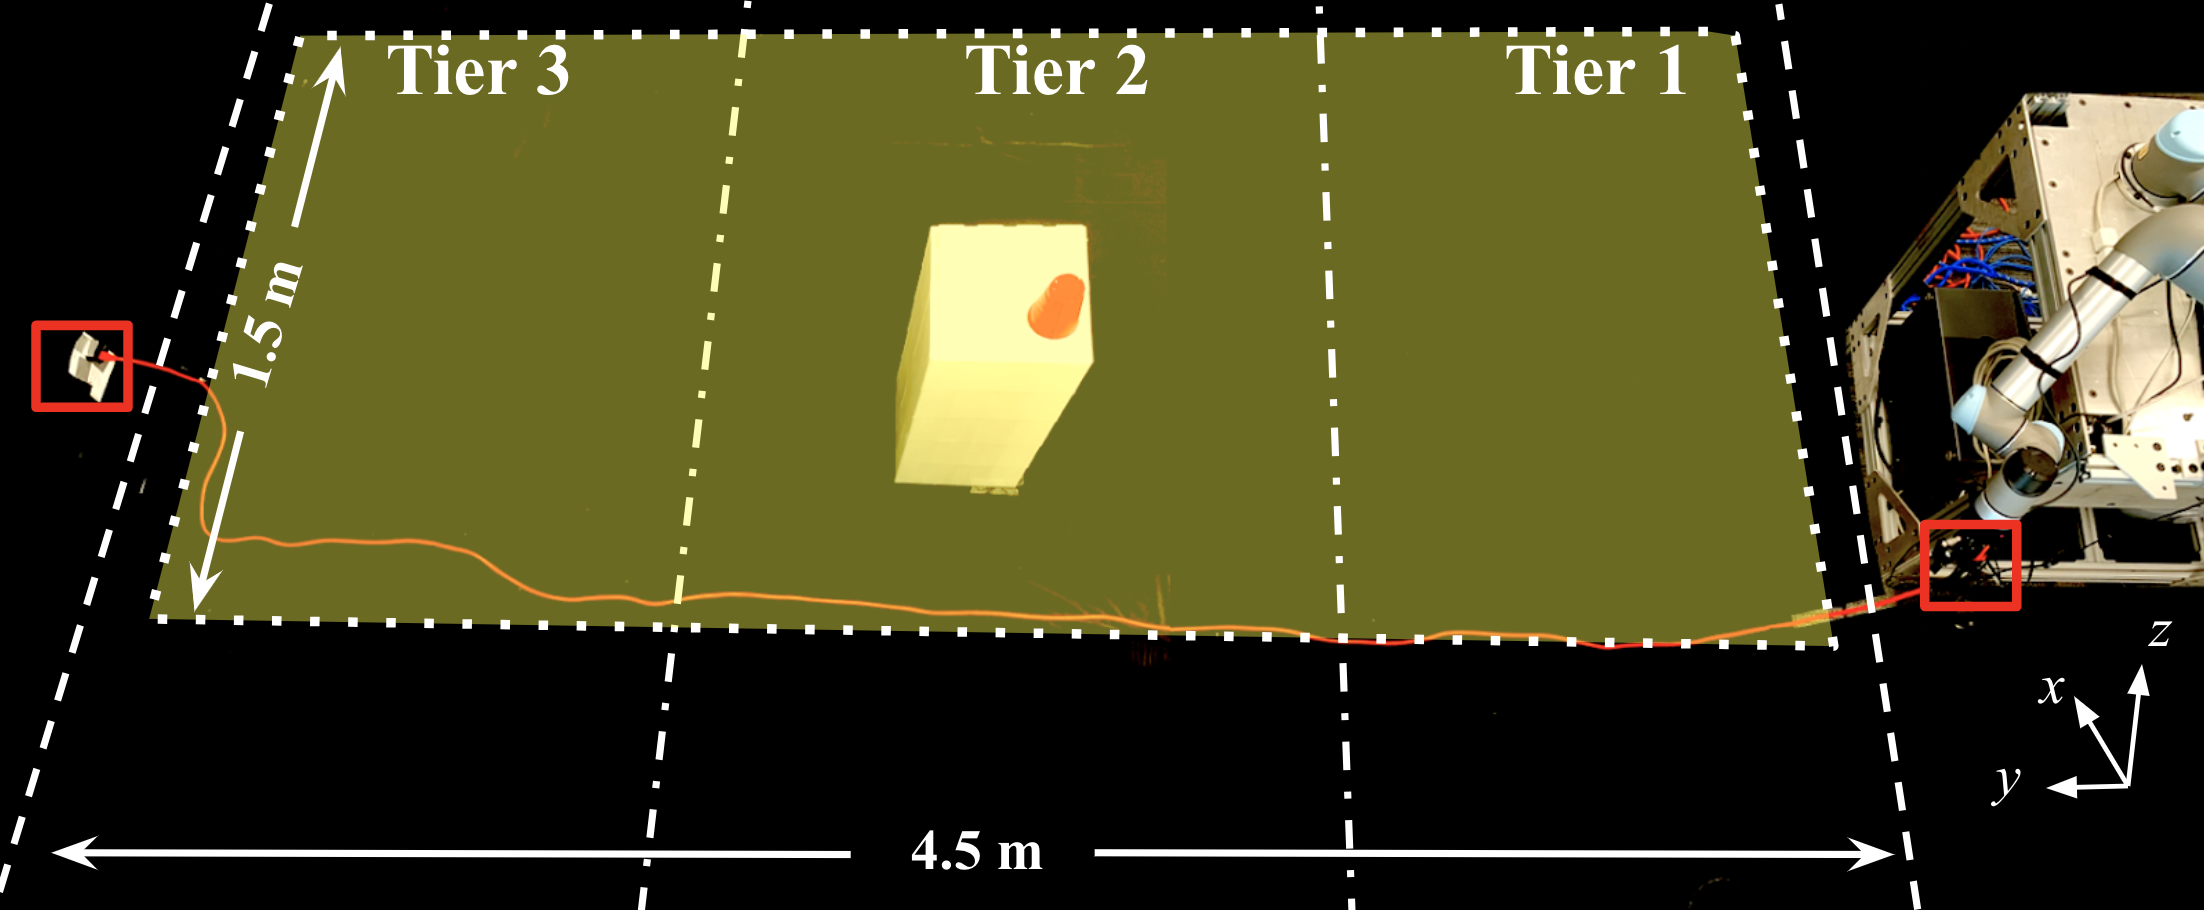
\includegraphics[width=\linewidth]{figures/layout.png}
    \caption{Design of physical experiments. We randomize the white Lego bricks' location within the yellow shaded area for vaulting and knocking. The yellow shaded area is also broken down into three difficulty tiers. Here we show an example of knocking, where the white Lego bricks form a base for the red target object on top of it and the robot aims to knock over the red target. \harry{TODO: prof. G said rotate. need to find a better way to convey the idea.}}
    \vspace*{-10pt}
    \label{fig:layout}
\end{figure}